\documentclass[11pt,letterpaper]{article}
\usepackage[utf8]{inputenc}
\usepackage[T1]{fontenc}
\usepackage[spanish,es-tabla]{babel}
\usepackage{lmodern,microtype,geometry,graphicx,booktabs,longtable,array,xcolor,hyperref,fancyhdr,float}
\geometry{margin=2.5cm,headheight=15pt}
\definecolor{navy}{HTML}{14364D}
\hypersetup{hypertexnames=false,colorlinks=true,linkcolor=navy,urlcolor=navy,pdftitle={EVA02 - MongoDB y PostgreSQL JSONB},pdfauthor={Luis Alberto Nafate Hernandez}}
\pagestyle{fancy}\fancyhf{}\fancyhead[L]{\small Bases de Datos en la Nube}\fancyhead[R]{\small EVA02}\fancyfoot[C]{\thepage}
\setlength{\parskip}{5pt}\setlength{\parindent}{0pt}\setlength{\emergencystretch}{2em}
\begin{document}
\begin{titlepage}\centering
{\Large\bfseries Universidad Politécnica de Chiapas\par}\vspace{.5cm}
{\large Ingeniería en Tecnologías de la Información\\e Innovación Digital\par}
\vspace{2cm}
{\Huge\bfseries\color{navy} Medición de métricas\\en bases documentales\par}\vspace{.7cm}
{\Large MongoDB frente a PostgreSQL JSONB\\bajo contención de CPU y memoria\par}
\vspace{1.1cm}{\large Evaluación 2026.C3.EVA02\par}
\vspace{1.4cm}
\begin{tabular}{rl}
\textbf{Alumno:}&Luis Alberto Nafate Hernandez\\[5pt]
\textbf{Matrícula:}&243728\\[5pt]
\textbf{Profesor:}&Horacio Irán Solís Cisneros\\[5pt]
\textbf{Materia:}&Bases de Datos en la Nube\\[5pt]
\textbf{Grupo y periodo:}&7B -- 2026.C3
\end{tabular}
\vfill
{\large\bfseries REPORTE TÉCNICO EXPERIMENTAL\par}\vspace{.3cm}
{\small 162 corridas originales y 3 verificaciones complementarias.\\Resultados, incidentes y limitaciones documentados.\par}
\vspace{.5cm}{1 de noviembre de 2026\par}
\end{titlepage}
\pagenumbering{roman}\tableofcontents\clearpage\pagenumbering{arabic}
\section{Especificaciones del host y del entorno Docker}
\subsection{Plataforma de ejecución}
El experimento compara agregaciones sobre el mismo conjunto documental, alojado en MongoDB y en una tabla PostgreSQL con JSONB. El cliente de carga corre en Windows; los servicios se ejecutan en la máquina virtual Linux de Docker Desktop. Las métricas del host Linux corresponden a esa máquina virtual, no a todos los procesos de Windows.
\begin{table}[H]\centering\small
\begin{tabular}{p{4.4cm}p{10cm}}\toprule
Elemento & Especificación observada\\\midrule
CPU & AMD Ryzen 5 7640HS; 6 núcleos y 12 procesadores lógicos; frecuencia máxima reportada por WMI: 4301 MHz. No se verificó por separado la frecuencia boost de fabricante.\\
RAM física & 40 GiB, módulos de 8 y 32 GiB, tipo SMBIOS 34 (DDR5). Las velocidades reportadas de los módulos no prueban la velocidad efectiva conjunta.\\
Almacenamiento & Unidades SSD NVMe Predator GM7 de 1 TB y Kioxia de 512 GB. No se verificó en este informe la ubicación física del VHDX de Docker.\\
Sistema & Windows 11 Home Single Language, versión 10.0.26300.\\
Virtualización & WSL 2.7.12.0; kernel 6.18.33.2 de WSL2; cgroups v2.\\
Docker & Desktop 4.87.0; Engine 29.7.2; Compose 5.4.0.\\
Recursos VM & 12 CPU lógicas y aproximadamente 19.1 GiB disponibles al diagnóstico inicial.\\\bottomrule
\end{tabular}\caption{Entorno medido; fuente: registros locales de hardware y Docker.}\end{table}
MongoDB verificado: 8.0.34. PostgreSQL verificado: PostgreSQL 17.11 (Debian 17.11-1.pgdg13+2) on x86\_64-pc-linux-gnu, compiled by gcc (Debian 14.2.0-19) 14.2.0, 64-bit. Los digests y la configuración efectiva están conservados en las evidencias del proyecto. Las versiones se fijaron para reproducibilidad; no se afirma que sean la versión estable más reciente a la fecha de entrega.
\subsection{Configuración y límites}
Se definieron tres perfiles: A con 4 CPU y 4096 MiB; B con 2 CPU y 2048 MiB; C con 1 CPU y 1024 MiB. El límite combinado de RAM y swap se igualó al de RAM para impedir swap por contenedor. No se utilizó \texttt{mem\_swappiness}, propiedad sin equivalencia directa por cgroup v2. Sólo se ejecuta un motor bajo prueba a la vez.
PostgreSQL se ejecuta con registro de archivos temporales y \texttt{work\_mem} de 4 o 64 MB según variante. Tras detectar el límite auxiliar de 64 MiB de memoria compartida de Docker, se configuró \texttt{shm\_size=1gb}; no es una reserva y el consumo sigue sometido al límite del perfil. Los resultados anteriores a ese cambio están identificados para repetición. MongoDB utiliza WiredTiger, sin sharding.
\section{Método de medición y verificación del baseline}
\subsection{Datos, consultas y comparabilidad}
Se generaron 500\,000 órdenes deterministas con semilla 2026 y tres ítems por orden. Incluyen UUID, fecha UTC canónica, cliente y geografía, ítems, pago y metadatos. Se cargó el mismo lote lógico en ambos motores. Se verificó el conteo completo y un hash canónico ordenado por identificador, excluyendo el identificador interno de MongoDB.
\textbf{SHA-256 canónico de comparación:} \par{\footnotesize\ttfamily 0bdef0102504460da70afde7e67ca3e6\ 111ff0f363b984fc867ab815ef070194}\par
Q1 desanida ítems, filtra precios mayores de 50 y agrupa por país y categoría, calculando suma, promedio y conteo. Se verificaron doce grupos equivalentes, con tolerancia relativa de $10^{-9}$ en valores numéricos. Q2 filtra pagos completados desde el 1 de enero de 2026 y obtiene los mil mayores totales; se verificaron los mil valores ordenados. Los identificadores del borde pueden variar ante empates.
MongoDB tiene índices simples en fecha e identificador. PostgreSQL tiene clave primaria UUID e índice de texto sobre la fecha extraída. El cast directo a \texttt{timestamptz} propuesto en el material no es una expresión inmutable para indexación; se empleó texto ISO UTC canónico de longitud fija en índice y predicado. La equivalencia es específica de ese formato, no se generaliza a husos u otras representaciones.
\subsection{Matriz y ciclo de vida}
La matriz explícita del playbook es $2\times3\times2\times3\times3=108$ corridas. Se amplió Q2 para medir ambas variantes en los tres perfiles, añadiendo 54 y llegando a 162. Esta ampliación es una decisión metodológica documentada, no un total expresamente escrito en el playbook.
Cada corrida contempla limpieza de caché del kernel Docker Desktop, calentamiento de 60 segundos, observación de 300 segundos y enfriamiento de 60 segundos. Los clientes consumen el resultado completo. Una barrera coordina el inicio tras preparar las conexiones. El generador usa hilos con conexiones independientes para carga de entrada/salida; esto es una adaptación al cliente Python y no una implementación multiproceso por cliente.
Las consultas tienen límite de 300 segundos. Para no bloquear la matriz se añadieron fases en procesos aislados y un máximo de 900 segundos por ejecutor. Los cambios del cliente se registran porque modifican la recuperación ante fallos. El tiempo total real puede superar siete minutos por drenado, preparación y recuperación. Se realizaron pausas solicitadas por el usuario y hubo una hibernación; los intentos afectados se conservan y revisan aparte.
\subsection{Definición de las métricas y sesgos}
QPS divide las consultas exitosas completadas dentro de la ventana entre 300 segundos. P50, P95 y P99 se calculan por interpolación lineal sobre latencias individuales exitosas. Las consultas que terminan fuera de la ventana están censuradas; por ello estos percentiles no describen todos los trabajos iniciados ni incluyen tiempos de fallos. Un promedio de P99 por corrida tampoco equivale al P99 combinado de todas las muestras.
Prometheus consulta cada segundo. Se extrae el delta del contador CFS y el máximo RSS. Si faltan muestras suficientes o el contador se reinicia, la fila no se considera válida. El contador CFS puede sumar espera de varios hilos y superar los 300 segundos: no es tiempo de pared ni porcentaje de CPU.
El nombre baseline no demuestra ausencia de contención. El perfil A también tiene cuota y presentó throttling con concurrencia; por tanto se informa como referencia con cuota, no como baseline empíricamente libre de estrangulamiento.
\section{Resultados consolidados}
\subsection{Estado del conjunto original}
La matriz original reúne 162 filas: 127 con estado ok, 18 con spill, 15 con error y 2 con OOM. Este informe utiliza exclusivamente esas filas originales; se completaron tres verificaciones complementarias y se cancelaron las siete restantes por instrucción del usuario. La matriz original se mantiene como análisis principal: los suplementos no borran fallos ni sustituyen resultados para mejorar la comparación. El CSV completo reúne 165 observaciones y conserva los 14 campos oficiales.
Los errores de memoria compartida y de telemetría no se presentan como resultados intrínsecos del motor. Las filas error/OOM se conservan para estabilidad, pero se excluyen de promedios de rendimiento. Por tanto una celda con menos de tres repeticiones válidas no permite la misma inferencia que una completa. La tabla incluye el número válido para evitar ocultarlo.
\subsection{Tablas por motor}
Se reportan medias de las métricas por corrida; los archivos de resumen incluyen además mediana y desviación estándar. CFS está expresado en segundos, RSS en MB decimales y latencias en milisegundos. Un guion significa dato no disponible, no cero.

\subsubsection{MongoDB}
{\fontsize{7.5}{9}\selectfont\setlength{\tabcolsep}{3pt}
\begin{longtable}{llrrrrrrrr}
\toprule Perfil & Consulta & Cli. & $n$ & QPS & P50 & P95 & P99 & CFS & RSS\\\midrule\endfirsthead
\toprule Perfil & Consulta & Cli. & $n$ & QPS & P50 & P95 & P99 & CFS & RSS\\\midrule\endhead
\bottomrule\endfoot
A & Q1 & 1 & 3 & 0.65 & 1512.64 & 1653.98 & 1733.08 & 0.00 & 598.11\\
A & Q1 & 10 & 3 & 1.49 & 6605.53 & 6940.11 & 7161.67 & 1777.53 & 655.77\\
A & Q1 & 50 & 3 & 1.03 & 51367.62 & 55935.84 & 57688.59 & 2318.35 & 822.99\\
A & Q2\_disk & 1 & 3 & 1.25 & 838.71 & 969.52 & 1058.08 & 0.00 & 603.95\\
A & Q2\_disk & 10 & 3 & 5.56 & 1801.52 & 1963.12 & 2065.70 & 1766.63 & 631.82\\
A & Q2\_disk & 50 & 3 & 4.98 & 9834.48 & 14686.50 & 16862.24 & 2364.66 & 706.35\\
A & Q2\_nodisk & 1 & 3 & 1.28 & 778.63 & 904.99 & 945.13 & 0.00 & 602.28\\
A & Q2\_nodisk & 10 & 3 & 5.53 & 1809.54 & 1971.17 & 2032.78 & 1765.98 & 632.08\\
A & Q2\_nodisk & 50 & 3 & 4.98 & 9773.95 & 14531.18 & 16577.43 & 2370.51 & 705.22\\
B & Q1 & 1 & 3 & 0.62 & 1618.33 & 1684.08 & 1701.39 & 0.00 & 633.50\\
B & Q1 & 10 & 3 & 0.76 & 12431.52 & 17200.35 & 17563.93 & 2382.67 & 660.35\\
B & Q1 & 50 & 3 & 0.66 & 70881.53 & 79321.16 & 82881.70 & 2942.39 & 774.52\\
B & Q2\_disk & 1 & 3 & 0.63 & 1585.96 & 1760.92 & 1876.16 & 0.00 & 671.00\\
B & Q2\_disk & 10 & 2 & 1.63 & 5887.71 & 7653.99 & 8187.36 & 1790.90 & 665.42\\
B & Q2\_disk & 50 & 3 & 1.01 & 45262.08 & 50572.33 & 52649.81 & 2832.69 & 741.74\\
B & Q2\_nodisk & 1 & 3 & 0.64 & 1543.67 & 1741.02 & 1889.25 & 0.00 & 664.60\\
B & Q2\_nodisk & 10 & 3 & 1.59 & 6208.73 & 7361.78 & 7872.21 & 1885.59 & 676.58\\
B & Q2\_nodisk & 50 & 3 & 0.98 & 47096.52 & 52533.23 & 54675.92 & 2835.97 & 739.25\\
C & Q1 & 1 & 3 & 0.34 & 3514.79 & 4342.15 & 4500.13 & 11.11 & 407.71\\
C & Q1 & 10 & 3 & 0.13 & 61287.41 & 62891.13 & 63710.38 & 2707.53 & 390.95\\
C & Q1 & 50 & 3 & 0.22 & 151798.39 & 167867.55 & 175845.47 & 3231.11 & 575.09\\
C & Q2\_disk & 1 & 3 & 0.13 & 7340.89 & 7575.78 & 7948.68 & 19.90 & 427.55\\
C & Q2\_disk & 10 & 3 & 0.27 & 35366.45 & 37630.14 & 37661.24 & 1946.82 & 420.57\\
C & Q2\_disk & 50 & 0 & -- & -- & -- & -- & -- & --\\
C & Q2\_nodisk & 1 & 3 & 0.13 & 7322.45 & 7720.05 & 8088.63 & 20.02 & 421.33\\
C & Q2\_nodisk & 10 & 3 & 0.27 & 35183.82 & 39746.88 & 39759.32 & 1945.04 & 420.74\\
C & Q2\_nodisk & 50 & 0 & -- & -- & -- & -- & -- & --\\
\end{longtable}}
\clearpage

\subsubsection{PostgreSQL JSONB}
{\fontsize{7.5}{9}\selectfont\setlength{\tabcolsep}{3pt}
\begin{longtable}{llrrrrrrrr}
\toprule Perfil & Consulta & Cli. & $n$ & QPS & P50 & P95 & P99 & CFS & RSS\\\midrule\endfirsthead
\toprule Perfil & Consulta & Cli. & $n$ & QPS & P50 & P95 & P99 & CFS & RSS\\\midrule\endhead
\bottomrule\endfoot
A & Q1 & 1 & 3 & 0.24 & 4191.31 & 4412.28 & 4534.67 & 0.00 & 103.63\\
A & Q1 & 10 & 3 & 0.18 & 50829.92 & 65386.98 & 68287.98 & 216.19 & 584.41\\
A & Q1 & 50 & 0 & -- & -- & -- & -- & -- & --\\
A & Q2\_4MB & 1 & 2 & 11.19 & 88.49 & 100.03 & 104.63 & 0.00 & 9.95\\
A & Q2\_4MB & 10 & 3 & 9.52 & 894.92 & 1710.14 & 1809.72 & 1774.49 & 36.40\\
A & Q2\_4MB & 50 & 3 & 9.68 & 5556.32 & 6624.48 & 7068.29 & 1783.36 & 115.91\\
A & Q2\_64MB & 1 & 3 & 10.99 & 90.12 & 101.39 & 105.82 & 0.00 & 10.09\\
A & Q2\_64MB & 10 & 3 & 9.54 & 895.56 & 1706.38 & 1806.28 & 1770.40 & 36.33\\
A & Q2\_64MB & 50 & 3 & 9.64 & 5562.60 & 6676.63 & 7104.97 & 1789.07 & 115.35\\
B & Q1 & 1 & 3 & 0.28 & 3466.92 & 4254.29 & 4503.47 & 42.41 & 104.85\\
B & Q1 & 10 & 3 & 0.14 & 60986.82 & 78347.00 & 79152.87 & 232.24 & 583.21\\
B & Q1 & 50 & 0 & -- & -- & -- & -- & -- & --\\
B & Q2\_4MB & 1 & 3 & 7.51 & 123.48 & 164.49 & 169.23 & 254.90 & 10.26\\
B & Q2\_4MB & 10 & 3 & 4.78 & 1780.41 & 3433.99 & 3658.51 & 2303.08 & 35.69\\
B & Q2\_4MB & 50 & 3 & 4.85 & 10962.82 & 13297.18 & 14263.14 & 2337.14 & 114.96\\
B & Q2\_64MB & 1 & 3 & 7.48 & 124.15 & 165.04 & 169.96 & 255.12 & 10.05\\
B & Q2\_64MB & 10 & 3 & 4.76 & 1768.52 & 3466.58 & 3695.00 & 2313.54 & 35.47\\
B & Q2\_64MB & 50 & 3 & 4.85 & 10932.15 & 13221.15 & 14133.92 & 2297.60 & 114.82\\
C & Q1 & 1 & 3 & 0.13 & 7895.50 & 9076.47 & 9319.75 & 66.10 & 102.19\\
C & Q1 & 10 & 3 & 0.05 & 146938.03 & 168411.81 & 168773.47 & 319.23 & 579.29\\
C & Q1 & 50 & 0 & -- & -- & -- & -- & -- & --\\
C & Q2\_4MB & 1 & 3 & 4.35 & 210.09 & 283.83 & 295.45 & 548.62 & 9.70\\
C & Q2\_4MB & 10 & 3 & 2.57 & 3228.86 & 6587.31 & 7054.28 & 2619.61 & 35.42\\
C & Q2\_4MB & 50 & 3 & 2.43 & 21428.73 & 26785.32 & 28873.75 & 2600.24 & 114.94\\
C & Q2\_64MB & 1 & 3 & 4.25 & 234.08 & 284.49 & 287.87 & 545.15 & 10.09\\
C & Q2\_64MB & 10 & 3 & 2.42 & 3464.40 & 6997.23 & 7438.46 & 2595.13 & 36.03\\
C & Q2\_64MB & 50 & 3 & 2.53 & 20598.36 & 26067.40 & 28765.19 & 2595.58 & 114.92\\
\end{longtable}}
\subsection{Lectura con limitaciones}
Q1 y Q2 no son cargas intercambiables: una compara expansión y agregado, la otra selección y Top-K. Los casos de alta concurrencia con errores no permiten concluir superioridad por un QPS aparente de cero si no hubo una ventana válida de consultas completadas. La comparación publicada utiliza la matriz original, declara los cambios del entorno y muestra la cobertura válida por celda. Los suplementos se identifican por archivo y no se combinan silenciosamente con el bloque primario.
\subsection{Contrastes cuantitativos y estabilidad}
Para mongodb, Q1 con un cliente pasó de 0.653 QPS en A a 0.338 en C, una reducción de 48.3\%. Es una comparación descriptiva de los perfiles, que cambian CPU y RAM conjuntamente.

Para postgresql, Q1 con un cliente pasó de 0.236 QPS en A a 0.128 en C, una reducción de 45.8\%. Es una comparación descriptiva de los perfiles, que cambian CPU y RAM conjuntamente.

En la matriz primaria hubo 145 corridas completadas sin error terminal (127 ok y 18 spill), 15 error y dos OOM. La frecuencia agregada de error/OOM fue $17/162=10.49\%$; mezcla incidentes experimentales y del entorno, por lo que no representa una tasa intrínseca de fallo del motor. Los 18 spills ocurrieron en Q1 de PostgreSQL y constituyen resultados terminados, no errores. La serie original contiene 54 celdas al desagregar las variantes Q2; no son 54 consultas distintas.
Las medias de la tabla están condicionadas al éxito. En especial, una celda con cero repeticiones válidas se muestra sin percentiles: no se informa latencia cero ni superioridad por ausencia de muestras. Medianas y desviaciones estándar por celda se incluyen en el archivo de resumen para examinar variabilidad, sin sustituir la evidencia individual.
\section{Análisis gráfico}
Las figuras de esta versión proceden de la matriz original. Las tres verificaciones se presentan como suplemento separado, sin modificar estas figuras. No deben interpretarse como comparación controlada entre ejecuciones previas y posteriores a cambios del entorno.
\begin{figure}[H]\centering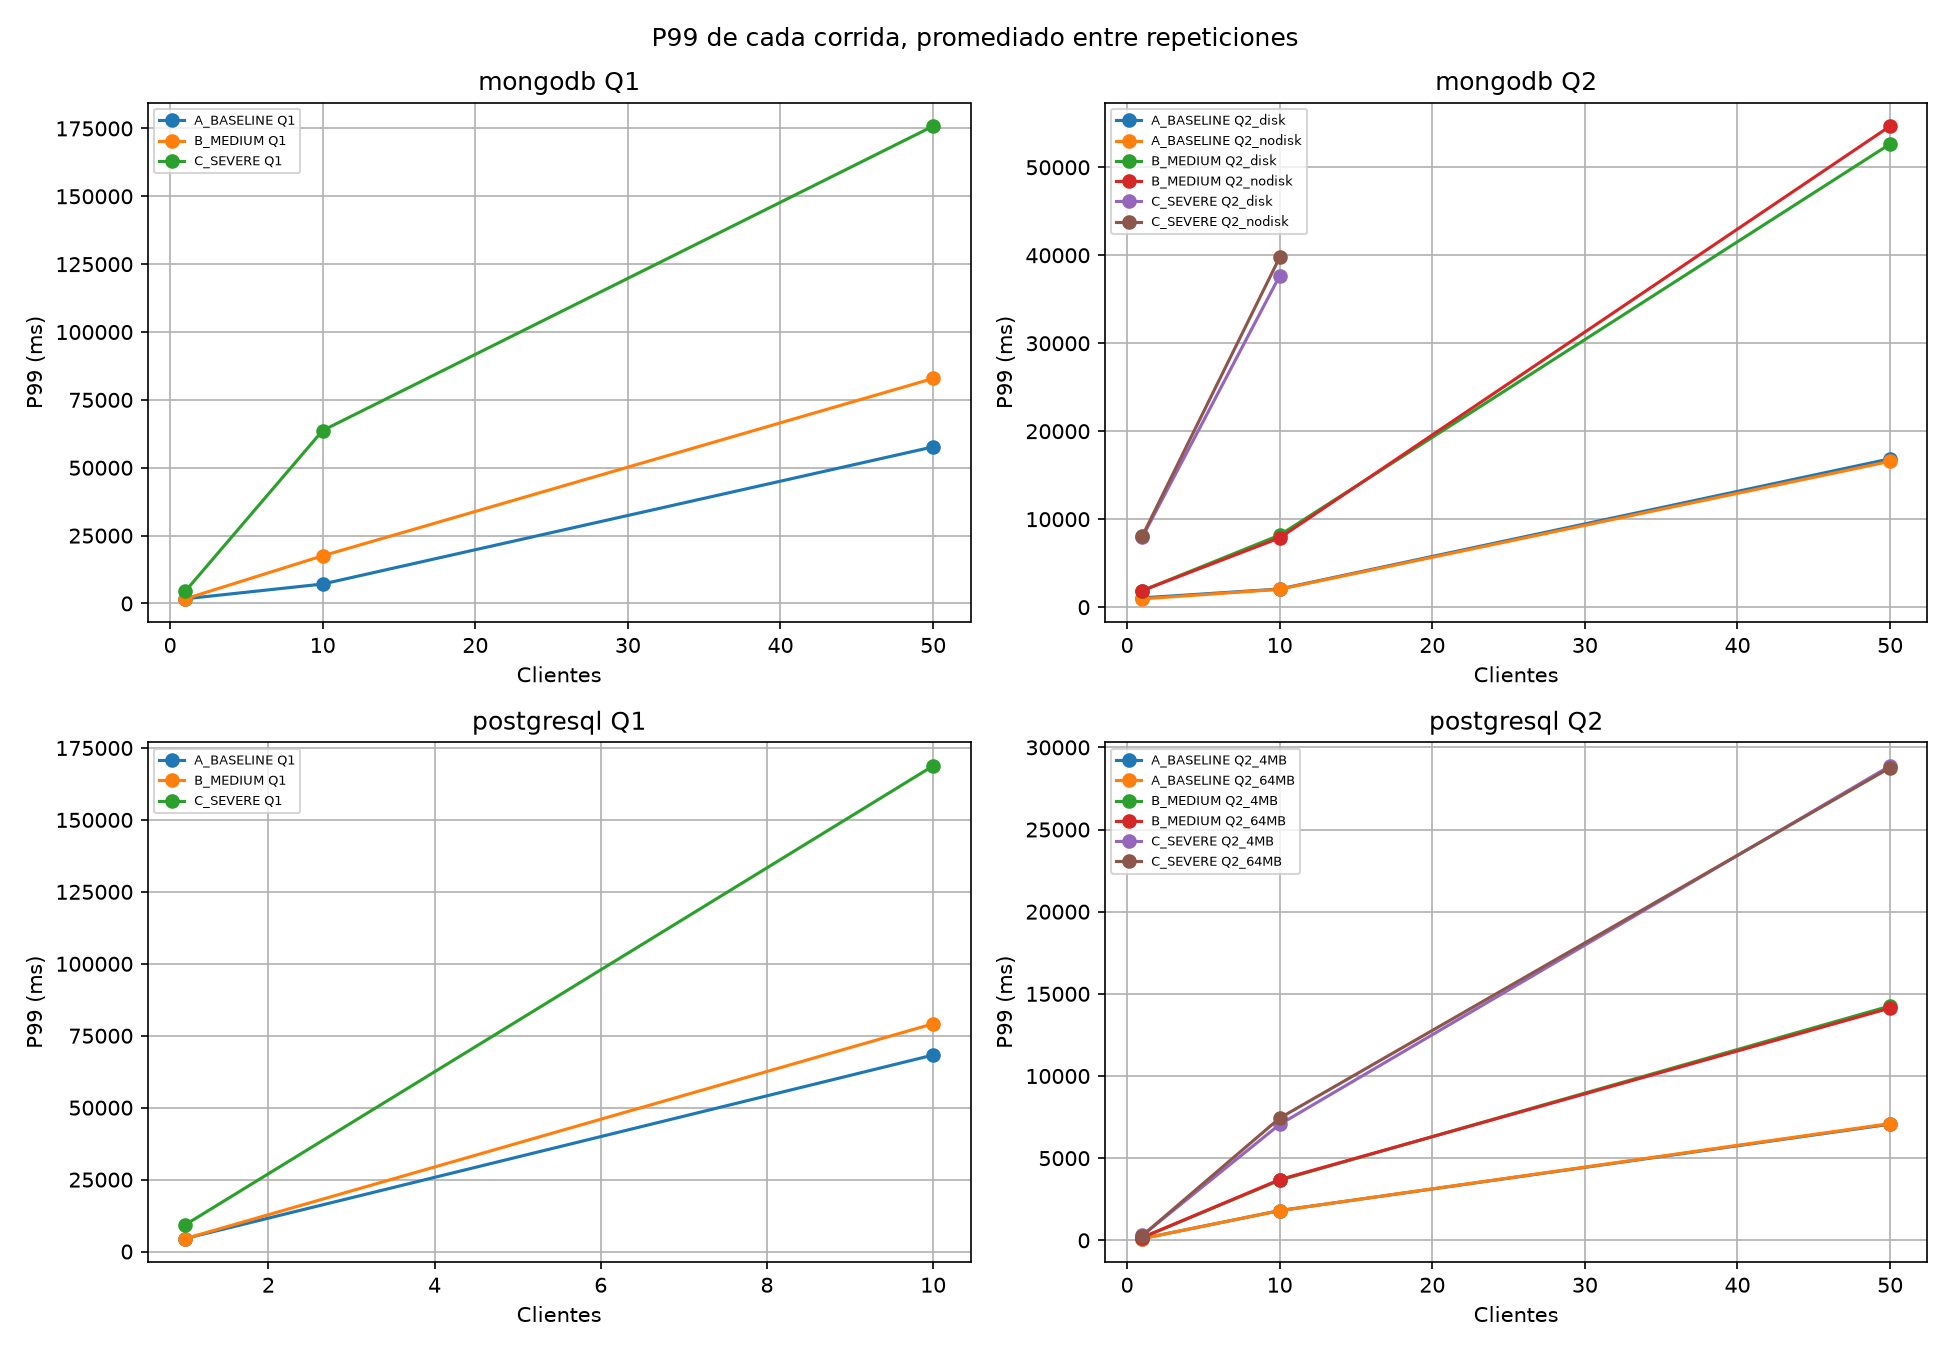
\includegraphics[width=\linewidth]{../p99_concurrencia.png}\caption{P99 frente a concurrencia. Cada línea resume percentiles por corrida; no es un percentil combinado.}\end{figure}
\begin{figure}[H]\centering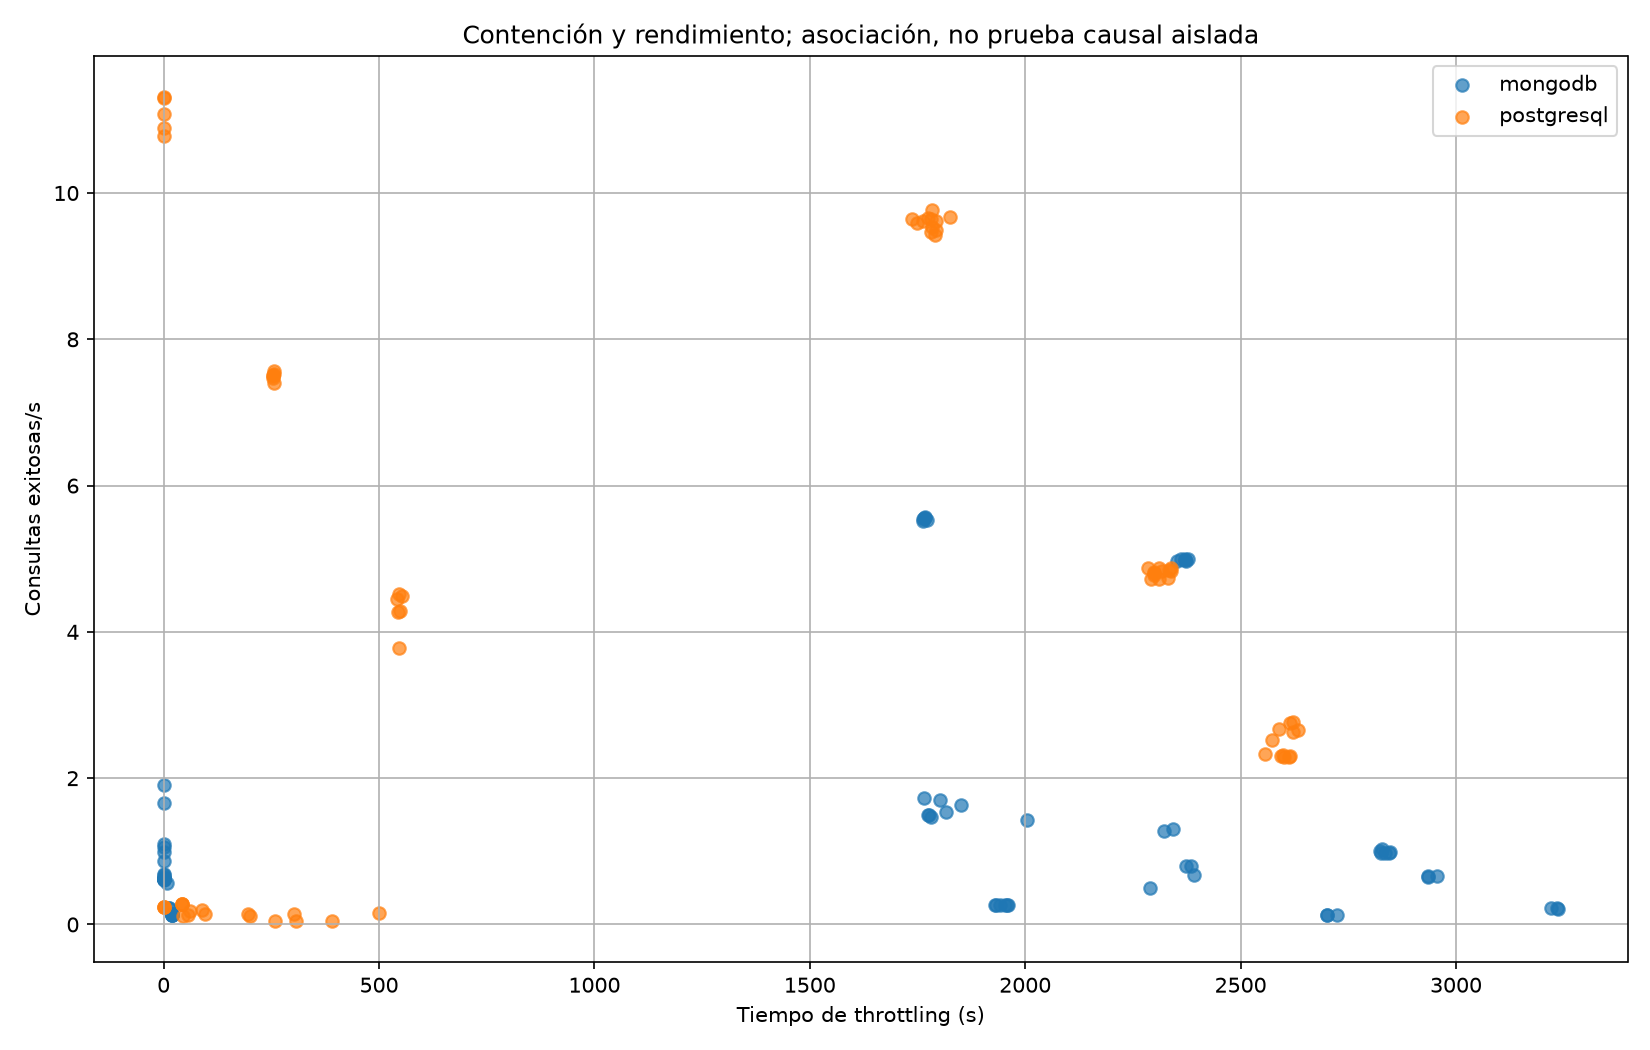
\includegraphics[width=\linewidth]{../throttling_qps.png}\caption{CFS y rendimiento. Los perfiles cambian CPU y RAM conjuntamente: una asociación no aísla causalidad.}\end{figure}
\begin{figure}[H]\centering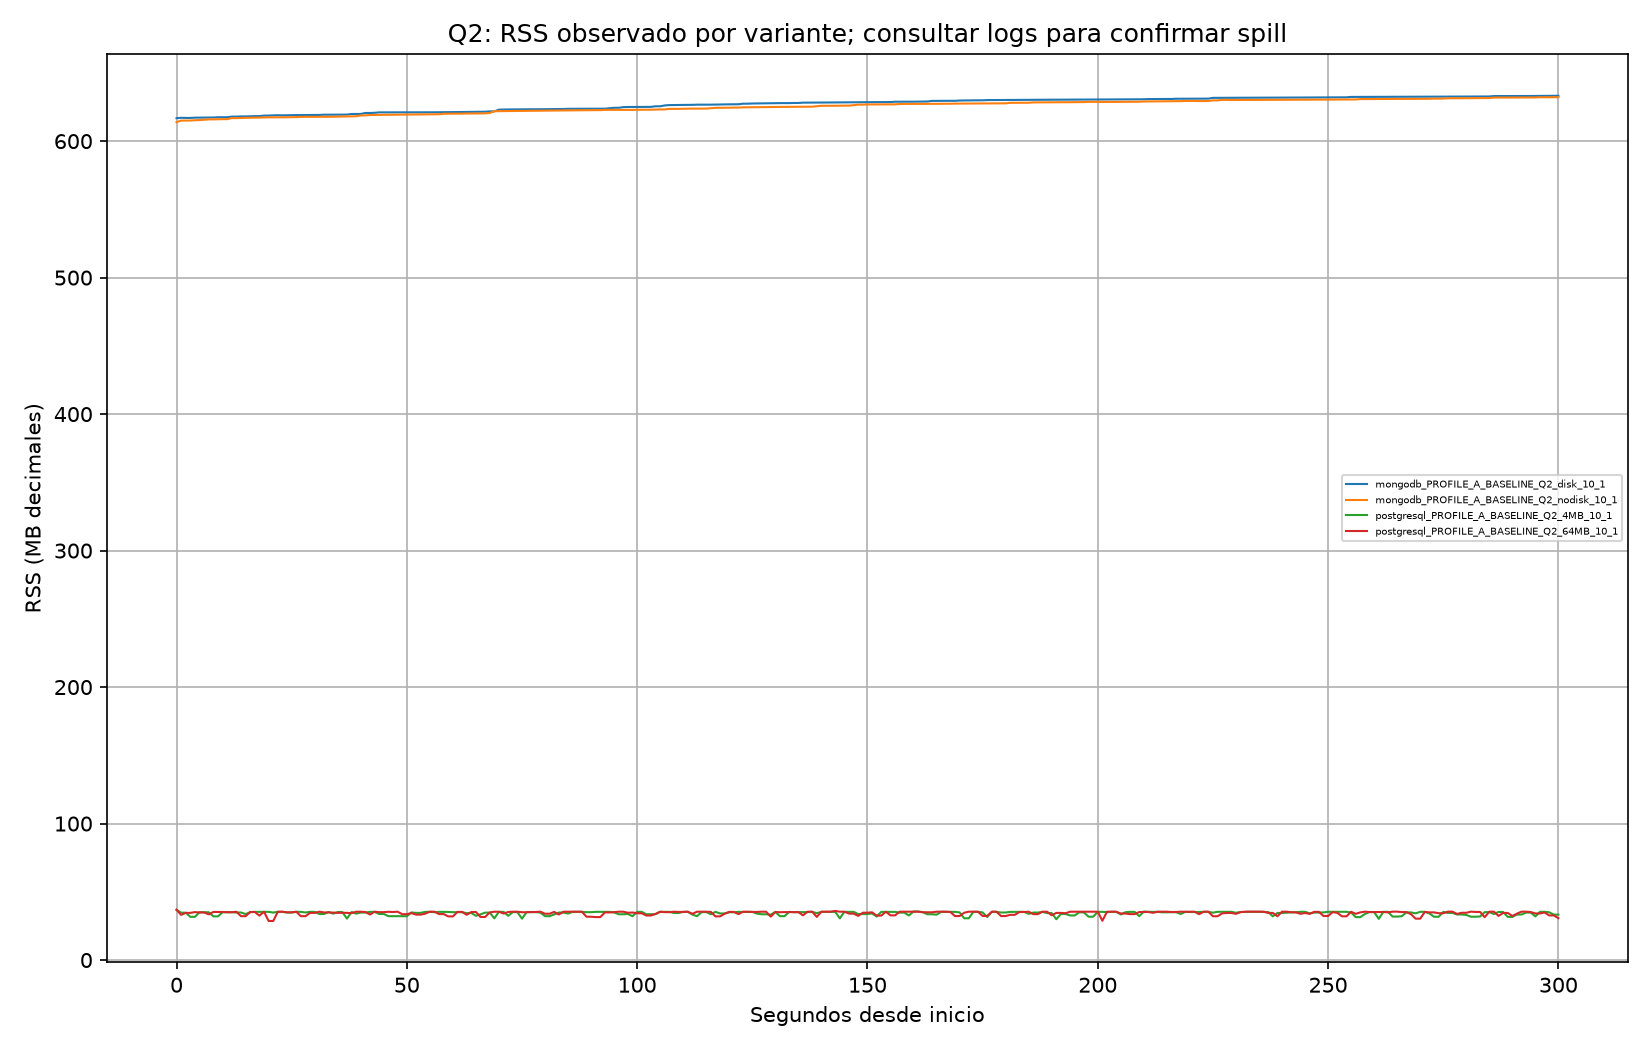
\includegraphics[width=\linewidth]{../rss_temporal.png}\caption{Series RSS de ejemplos Q2 por variante. Permitir disco no demuestra que haya ocurrido spill.}\end{figure}
\section{Planes de ejecución}
Se capturaron planes reales fuera de las ventanas: \texttt{executionStats} para MongoDB y \texttt{EXPLAIN (ANALYZE, BUFFERS, VERBOSE)} para PostgreSQL, con ambas variantes. Están en las evidencias de validación; los planes iniciales son del baseline y no prueban automáticamente los operadores de todos los perfiles.
Q1 permite estudiar el costo de recorrer órdenes, expandir arreglos y agrupar. La cantidad de filas expandidas es mayor que el número de órdenes. Q2 puede emplear una selección Top-K acotada en lugar de materializar un ordenamiento completo. Los operadores efectivos se detallan a continuación; no se deduce external merge sólo a partir de que se usaron 4 MB.
La evidencia de archivos temporales en PostgreSQL Q1 no se atribuye automáticamente al operador Sort: también puede proceder de otros operadores o materialización. El desglose siguiente identifica archivos y operadores realmente observados.

\subsection{Operadores y evidencia efectiva}
En \texttt{Q1\_mongo\_nodisk\_plan.json}, MongoDB examinó 500\,000 documentos con COLLSCAN, expandió 1\,500\,000 ítems y dejó 1\,254\,674 tras el filtro. El agrupamiento devolvió doce grupos con \texttt{usedDisk=false} y cero spills. El tiempo registrado en executionStats fue 1502 ms (1522 ms en la variante con disco permitido); el campo no debe confundirse con la latencia completa del cliente.
En \texttt{Q1\_postgres\_4MB\_plan.json} se observaron Aggregate, Incremental Sort, Nested Loop, Gather Merge, Seq Scan y Function Scan. El ordenamiento anterior a la expansión empleó external merge, con espacios de disco de 173248, 214864 y 196584 kB entre procesos. El tiempo total del plan fue 3122.06 ms. Con 64 MB también hubo external merge (3175.71 ms); elevar work\_mem no eliminó este volcado.
Q2 MongoDB utilizó IXSCAN, FETCH y SORT: examinó 247\,702 documentos, el filtro dejó 61\,738 y se devolvieron mil. No hubo spill en los dos planes; sus tiempos fueron 571 y 534 ms. Q2 PostgreSQL utilizó Seq Scan, Sort, Gather Merge y Limit; los Sort mostraron top-N heapsort en memoria con aproximadamente 271--275 kB por proceso. Los tiempos fueron 103.987 y 113.471 ms para 4 y 64 MB. Estos planes explican por qué Q2 no produjo el spill que se podría haber esperado sólo por su título de ordenamiento masivo.
La comparación tiene diferencias reales de estrategia: el plan MongoDB Q2 examinó menos documentos por el índice temporal, mientras PostgreSQL eligió lectura secuencial. Ningún resultado se atribuye exclusivamente al formato BSON o JSONB sin considerar esos planes.
\section{Interpretación: memoria, disco y throttling de cgroups}
\subsection{Presupuestos y estabilidad}
Las cuotas CPU pueden agotar el presupuesto periódico aunque el equipo tenga otros núcleos libres. La suma de espera entre hilos explica que CFS acumulado exceda la duración de la observación. El RSS de cAdvisor no equivale a toda la memoria imputada al cgroup; tampoco es intercambiable con la caché de páginas del host.
WiredTiger y las etapas de agregación tienen presupuestos distintos. En PostgreSQL, \texttt{work\_mem} es un presupuesto por operación y puede multiplicarse por conexiones y trabajadores. Un límite de contenedor no se convierte automáticamente en un presupuesto seguro para cincuenta clientes.
\subsection{Spill, OOM y errores de laboratorio}
Spill se registra mediante indicadores \texttt{usedDisk} o archivos temporales; OOM mediante estado Docker y sus evidencias. Un timeout o falta de memoria compartida no prueba un OOM. Las filas originales conservaron todos esos estados. En particular, el límite auxiliar de memoria compartida se corrigió y la pérdida de telemetría por cierre de cAdvisor obliga a repetir la observación.
El perfil severo PostgreSQL Q1 con 50 clientes produjo estados OOM en dos intentos registrados. Esto constituye evidencia de inestabilidad bajo esa configuración, no una afirmación de que el motor falle con cualquier documento o carga. Debe contrastarse con los logs e inspect conservados y con la recuperación aplicada.
\subsection{Alcance de las conclusiones}
Hay limitaciones explícitas: cliente Windows externo a la VM, posible carga del host, pausas y cambios del cliente, censura temporal de consultas lentas y falta de aleatorización de la secuencia. El estudio es descriptivo de esta plataforma; no generaliza directamente a servicios administrados en nube.
La pregunta de costo por mil documentos (M3) requiere CPU realmente consumida y documentos examinados, no sólo tiempo CFS y RSS máximo. Este informe no inventa ese costo a partir de los indicadores disponibles; no se establece una conclusión cuantitativa de M3 con la información reunida. Esta limitación no se subsana usando throttling como si fuera CPU consumida.
\section{Recomendaciones técnicas para despliegues documentales en la nube}
Conviene validar el motor contra las consultas, el modelo transaccional y los requisitos operativos reales. Estos resultados no establecen un ganador universal para todo JSON. PostgreSQL JSONB permite combinar documentos y relaciones; MongoDB ofrece un modelo documental nativo. La selección debe apoyarse en la carga y en los índices necesarios, además de la estabilidad observada.
Se recomienda dimensionar límites CPU observando P95/P99 y throttling, no sólo promedio de QPS; limitar concurrencia para evitar colas y presión de memoria; estimar el presupuesto de operaciones simultáneas antes de aumentar \texttt{work\_mem}; y verificar cuotas y memoria compartida en el contenedor antes de comparar motores.
En Kubernetes o ECS se deben comprobar los límites efectivos del despliegue y repetir el protocolo en la infraestructura objetivo. Los números de este equipo no son una recomendación certificada de tamaño de instancia. El siguiente paso es evaluar las mismas consultas en perfiles donde CPU y RAM varíen por separado, para aislar sus efectos.
\clearpage
\section*{Referencias y trazabilidad}\addcontentsline{toc}{section}{Referencias y trazabilidad}
\begin{enumerate}
\item Material académico de la evaluación: \textit{playbook.pdf}, secciones 1--8, y \textit{playbook\_sesion.pdf}. Copias originales conservadas en el proyecto.
\item MongoDB. \textit{Sort aggregation stage}, documentación de versión 8.0. \url{https://www.mongodb.com/docs/v8.0/reference/operator/aggregation/sort/}
\item PostgreSQL. \textit{CREATE INDEX}, documentación de versión 17. \url{https://www.postgresql.org/docs/17/sql-createindex.html}
\item Tectonic. \textit{Installing Tectonic}. Compilador portátil 0.17.0. \url{https://tectonic-typesetting.github.io/book/latest/installation/}
\end{enumerate}
\textbf{Archivos de evidencia:} CSV original, CSV de repeticiones, manifiesto de selección, comparación canónica de datos, planes, logs por corrida, inspect de contenedores, series Prometheus y muestras individuales. Todos los archivos de resultados deben conservar sus nombres y trazabilidad al reorganizar el repositorio.
\textbf{Criterio de cierre:} por instrucción del alumno se conserva el resultado completo, incluidos fallos de ejecución y de laboratorio. No se repiten indefinidamente las celdas hasta obtener éxito. El informe declara las limitaciones que impiden atribuir todos los errores a los motores o afirmar una comparación perfectamente controlada.
\clearpage\appendix
\section{Registro de fallos y problemas del experimento}
Las filas se numeran desde uno, excluyendo la cabecera del CSV original. Un timeout es un resultado de la configuración y del límite aplicado; no se equipara automáticamente con OOM. Las filas de fallos del entorno siguen visibles, pero no sustentan superioridad del motor.
{\small\begin{longtable}{r>{\raggedright\arraybackslash}p{3cm}>{\raggedright\arraybackslash}p{2.7cm}>{\raggedright\arraybackslash}p{6.5cm}}
\toprule Fila & Motor y perfil & Carga & Evidencia y clasificación\\\midrule\endfirsthead
\toprule Fila & Motor y perfil & Carga & Evidencia y clasificación\\\midrule\endhead\bottomrule\endfoot
48 & mongodb B & Q2\_disk, c=10, r=3 & Timeout/cancelación; el usuario informó hibernación. No atribuir exclusivamente al motor.\\
76 & mongodb C & Q2\_nodisk, c=50, r=1 & Timeout/cancelación de consulta; se conserva como resultado y no se afirma OOM.\\
77 & mongodb C & Q2\_disk, c=50, r=1 & Timeout/cancelación de consulta; se conserva como resultado y no se afirma OOM.\\
78 & mongodb C & Q2\_nodisk, c=50, r=2 & Timeout/cancelación de consulta; se conserva como resultado y no se afirma OOM.\\
79 & mongodb C & Q2\_disk, c=50, r=2 & Timeout/cancelación de consulta; se conserva como resultado y no se afirma OOM.\\
80 & mongodb C & Q2\_nodisk, c=50, r=3 & Timeout/cancelación de consulta; se conserva como resultado y no se afirma OOM.\\
81 & mongodb C & Q2\_disk, c=50, r=3 & Timeout/cancelación de consulta; se conserva como resultado y no se afirma OOM.\\
88 & postgresql A & Q1, c=50, r=1 & Memoria compartida auxiliar de Docker agotada; problema de configuración, no prueba de OOM.\\
89 & postgresql A & Q1, c=50, r=2 & Timeout/cancelación de consulta; se conserva como resultado y no se afirma OOM.\\
90 & postgresql A & Q1, c=50, r=3 & Timeout/cancelación de consulta; se conserva como resultado y no se afirma OOM.\\
95 & postgresql A & Q2\_4MB, c=1, r=3 & cAdvisor terminó; ventana incompleta. Se conservan las métricas vacías sin interpolación.\\
115 & postgresql B & Q1, c=50, r=1 & Timeout/cancelación de consulta; se conserva como resultado y no se afirma OOM.\\
116 & postgresql B & Q1, c=50, r=2 & Timeout/cancelación de consulta; se conserva como resultado y no se afirma OOM.\\
117 & postgresql B & Q1, c=50, r=3 & Timeout/cancelación de consulta; se conserva como resultado y no se afirma OOM.\\
142 & postgresql C & Q1, c=50, r=1 & Docker inspect registró OOMKilled; evidencia de agotamiento bajo el límite aplicado.\\
143 & postgresql C & Q1, c=50, r=2 & Docker inspect registró OOMKilled; evidencia de agotamiento bajo el límite aplicado.\\
144 & postgresql C & Q1, c=50, r=3 & Control externo del cliente activado; muestras o fase incompletas. No tratar como throughput cero medido.\\
\end{longtable}}
Los intentos interrumpidos por pausas del usuario o por bloqueo, sin ventana completa, se conservan en evidencias/interrumpidas. No se fabricó una fila de medición por cada carpeta vacía o incompleta. El CSV de todas las pruebas contiene sólo las 165 observaciones que llegaron a escribirse; no puede representar latencias no medidas.
\subsection{Problemas del entorno y controles incorporados}
Se documentaron hibernación, memoria compartida inicial de 64 MiB, cierre de cAdvisor y bloqueo del cliente. Las correcciones fueron: memoria compartida máxima de 1 GiB; reinicio de cAdvisor; timeout de conexión de quince segundos; opciones de sesión en conexión; procesos de carga aislados; y corte externo de 900 segundos por ejecutor con terminación del árbol de procesos. El conjunto primario contiene más de una versión del cliente; esta condición limita la comparabilidad de fallos y se declara en lugar de ocultarse.
\section{Verificaciones complementarias y archivos de entrega}
Se completaron tres de diez verificaciones planeadas. Las restantes se cancelaron por instrucción del alumno para cerrar el estudio conservando los fallos como evidencia. No se afirma que todas las incidencias del entorno hayan sido reejecutadas bajo una configuración homogénea.
\begin{center}\small\begin{tabular}{llrrr}\toprule Motor & Carga & Clientes & QPS & P99 (ms)\\\midrule
mongodb & Q2\_disk & 10 & 1.143 & 11495.43\\
postgresql & Q1 & 1 & 0.367 & 4251.66\\
postgresql & Q1 & 1 & 0.333 & 4444.01\\
\bottomrule\end{tabular}\end{center}
Los archivos oficiales son: CSV de todas las observaciones con 14 columnas; matriz primaria original; suplemento de verificaciones; manifiesto de cierre; resumen con media, mediana y desviación; fuentes de consulta y generación; Compose y telemetría; planes; logs y muestras individuales; fuente LaTeX, PDF y guía para exposición. El repositorio conserva etiquetas de versión para esta entrega, sin publicación remota automática.
\end{document}
